\documentclass[aspectratio=169]{beamer}

\usepackage{DejaVuSansMono}
\usepackage[utf8]{inputenc}
\usepackage[T1]{fontenc}

\usepackage{amsmath}
\usepackage{wasysym}

\usepackage{listings}
\usepackage{lstautogobble}
\lstdefinestyle{cpp}{
  autogobble,
  basicstyle=\ttfamily\footnotesize,
  keywordstyle=\color{blue},
  commentstyle=\color{gray},
  language=c++,
  mathescape,
  literate={∷}{{:\!\!:}}1
           {←}{{\csname u8:\detokenize{←}\endcsname}}1
           {→}{{\csname u8:\detokenize{→}\endcsname}}1
           {↓}{{\csname u8:\detokenize{↓}\endcsname}}1
           {↑}{{\csname u8:\detokenize{↑}\endcsname}}1,
  columns=fullflexible,
  keepspaces
}
\lstdefinestyle{haskell}{
  autogobble,
  basicstyle=\ttfamily\footnotesize,
  morecomment=[l]{--},
  morekeywords={data},
  keywordstyle=\color{blue},
  commentstyle=\color{gray},
  mathescape,
  literate={∷}{{:\!\!:}}1
           {←}{{\csname u8:\detokenize{←}\endcsname}}1
           {→}{{\csname u8:\detokenize{→}\endcsname}}1
           {↓}{{\csname u8:\detokenize{↓}\endcsname}}1
           {↑}{{\csname u8:\detokenize{↑}\endcsname}}1,
  columns=fixed,
  keepspaces
}
\lstnewenvironment{cppcode}{\lstset{style=cpp}}{}
\lstnewenvironment{haskellcode}{\lstset{style=haskell}}{}
\newcommand{\cppinline}[1]{\lstinline[style=cpp]!#1!}
\newcommand{\haskellinline}[1]{\lstinline[style=haskell]!#1!}

\newcommand{\halcheck}{\texttt{halcheck}}

\title{\halcheck}
\author{Anthony Vandikas}
\date{December 22, 2023}
\usetheme{metropolis}

\begin{document}

\frame{\titlepage}

\begin{frame}{\halcheck{} --- Overview}
  \tableofcontents
\end{frame}

\section{Overview}

\begin{frame}<1>[label=overview]{\halcheck{} --- Overview \only<4>{--- Summary}}
  \begin{block}{Why \halcheck?}
    \begin{enumerate}
      \item<alert@1> First-order(ish) API
      \item<alert@2> Support for custom test-case generation strategies
      \item<alert@3> Better space complexity
    \end{enumerate}
  \end{block}
\end{frame}

\begin{frame}[fragile]{\halcheck{} --- Overview --- API}
  All PBT frameworks are direct ports or descendants of QuickCheck. These frameworks all consist of:

  \bigskip{}
  \pause{}

  \begin{columns}[T,onlytextwidth]
    \begin{column}{0.47\textwidth}
      \begin{block}{A central generator data type:}
        \begin{haskellcode}
          --     Source of
          --     randomness ↓
          data Gen a = Gen (Random → a)
        \end{haskellcode}
      \end{block}
    \end{column}

    \pause{}

    \begin{column}{0.53\textwidth}
      \begin{block}{A set of basic combinators:}
        \begin{haskellcode}
          choose    ∷ (Int, Int) → Gen Int
          suchThat  ∷ (a → Bool) → Gen a → Gen a
          frequency ∷ [(Int, Gen a)] → Gen a
          ...
        \end{haskellcode}
      \end{block}
    \end{column}
  \end{columns}

  \pause{}

  \bigskip{}

  \begin{itemize}
    \item Users must be comfortable reasoning about higher-order functions.
    \item Users must ensure generators are only invoked in the \alert{correct context}.
  \end{itemize}
\end{frame}

\begin{frame}[fragile,t]{\halcheck{} --- Overview --- API}
  \textbf{Example:} \emph{Write a generator combinator that produces \cppinline{std::vector}s up to (but not including) a given length.}

  \begin{onlyenv}<+>
    \begin{cppcode}
      // RapidCheck
      Gen<std::vector<int>> example(int N) {
        return gen::container<std::vector<int>>(
          *gen::inRange(0, N),
          gen::arbitrary<int>);
      }
    \end{cppcode}

    \begin{haskellcode}
      -- QuickCheck
      example n = vectorOf (choose (0, n - 1)) arbitrary
    \end{haskellcode}
  \end{onlyenv}

  \begin{onlyenv}<+>
    \begin{cppcode}
      // RapidCheck
      Gen<std::vector<int>> example(int N) {
        return gen::container<std::vector<int>>(
          *gen::inRange(0, N), // WRONG (no compiler error)
          gen::arbitrary<int>);
      }
    \end{cppcode}

    \begin{haskellcode}
      -- QuickCheck         ↓ WRONG (compiler error)
      example n = vectorOf (choose (0, n - 1)) arbitrary
    \end{haskellcode}
  \end{onlyenv}

  \begin{onlyenv}<+>
    \begin{cppcode}
      // RapidCheck
      Gen<std::vector<int>> example(int N) {
        // WRONG: n is computed $\mathbf{once}$, $\mathit{before}$ calling container
        auto n = *gen::inRange(0, N);
        return gen::container<std::vector<int>>(n, gen::arbitrary<int>());
      }
    \end{cppcode}
    \begin{haskellcode}
      -- QuickCheck         ↓ WRONG: choose ∷ (Int, Int) → $\color{red}{\mathtt{Gen\ Int}}$
      example n = vectorOf (choose (0, n - 1)) arbitrary
      --          ↑ WRONG: vectorOf ∷ $\color{red}{\mathtt{Int}}$ → Gen Int → Gen [Int]
    \end{haskellcode}
  \end{onlyenv}

  \begin{onlyenv}<+>
    \textbf{Solution:} Delay computation of \cppinline{*gen::inRange(0, N)} using \cppinline{gen::exec}.

    \begin{columns}[T,onlytextwidth]
      \column{0.53\textwidth}
      \begin{cppcode}
        // RapidCheck
        Gen<std::vector<int>> example(int N) {
          return gen::exec([=] {
            return *gen::container<std::vector<int>>(
              *gen::inRange(0, N),
              gen::arbitrary<int>);
          });
        }
      \end{cppcode}

      \column{0.35\textwidth}
      \begin{haskellcode}
        -- QuickCheck
        example n = do
          i <- choose (0, n - 1)
          vectorOf i arbitrary
      \end{haskellcode}
    \end{columns}
  \end{onlyenv}
\end{frame}

\begin{frame}[fragile]{\halcheck{} --- Overview --- API}
  \begin{itemize}
    \item \textbf{Problem:} Need to ensure generators are only invoked in the correct context.
          \begin{itemize}
            \item Haskell's type system ensures this always happens.
            \item C++'s type system can provide no such guarantee!
          \end{itemize}
          \pause{}
    \item \textbf{Solution:} Get rid of the generator type!
          \begin{itemize}
            \item All code is written in the generator context.
            \item Bonus: fewer higher-order functions.
          \end{itemize}
  \end{itemize}

  \begin{cppcode}
    // halcheck
    std::vector<int> example(int N) {
      return gen::container<std::vector<int>>(
        gen::range(0, N),
        gen::arbitrary<int>);
    }
  \end{cppcode}
\end{frame}

\againframe<2>{overview}

\begin{frame}{\halcheck{} --- Overview --- Strategies}
  There are various desirable strategies for generating data:
  \begin{itemize}
    \item Random (almost everything)
    \item Enumerative (SmallCheck/LeanCheck) \pause{}
    \item Learning-based (RLCheck)
    \item Coverage-guided (FuzzTest) \pause{}
  \end{itemize}

  Most PBT frameworks (and all C++ PBT frameworks) use a \alert{fixed strategy}.
\end{frame}

\begin{frame}[fragile]{\halcheck{} --- Overview --- Strategies}
  \halcheck{} provides combinators for specifying strategies:

  \begin{cppcode}
    //   random(int) → strategy
    // ↓ Executes random test cases forever or until a bug is found.
    test::random(seed)([] { /* test code */ });
  \end{cppcode}

  \pause{}

  \begin{cppcode}
    //   ordered(strategy) → strategy
    // ↓ Executes all test cases in order, from smallest to largest.
    test::ordered()([] { /* test code */ });
  \end{cppcode}

  \pause{}

  \begin{cppcode}
    //   limit(strategy, int) → strategy
    //   shrink(strategy) → strategy
    //   Executes at most 100 random test cases.
    // ↓ Performs shrinking if an exception is thrown.
    test::shrink(test::limit(test::random(), 100))([] { /* test code */ });
  \end{cppcode}

  \pause{}

  (Intended for advanced users.)
\end{frame}

\againframe<3>{overview}

\begin{frame}[fragile]{\halcheck{} --- Overview --- Space Complexity}
  \begin{columns}[t,onlytextwidth]
    \column{0.5\textwidth}
    \begin{block}{How does shrinking work?}
      \bigskip

      Internally, every generator is a function returning a ``shrink tree'' of values.

      \bigskip

      \begin{haskellcode}
        data Gen a = Gen (Random → Tree a)
      \end{haskellcode}

      Shrink trees can be \alert{very large} so they must be computed lazily.
    \end{block}

    \column{0.5\textwidth}
    \begin{block}{Shrink tree for a list:}
      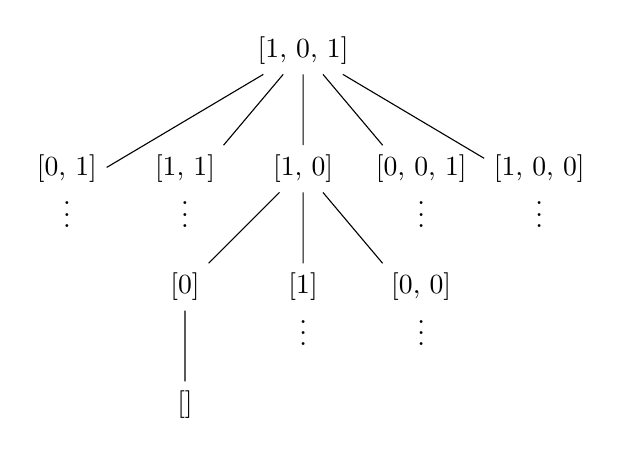
\begin{tikzpicture}[align=center,anchor=north,level distance=1.2cm]
        \node{[1, 0, 1]}
        child {node {[0, 1]\\\vdots}}
        child {node {[1, 1]\\\vdots}}
        child {node {[1, 0]}
            child {node {[0]}
                child {node {[]}}}
            child {node {[1]\\\vdots}}
            child {node {[0, 0]\\\vdots}}}
        child {node {[0, 0, 1]\\\vdots}}
        child {node {[1, 0, 0]\\\vdots}}
        ;
      \end{tikzpicture}
    \end{block}
  \end{columns}

  \pause{}

  This implementation strategy \alert{does not work for C++!}
\end{frame}

\begin{frame}[fragile]{\halcheck{} --- Overview --- Space Complexity}
  \begin{block}{Example:}
    \begin{cppcode}
      auto xs = *gen::arbitrary<std::vector<int>>();
      auto x  = *gen::elementOf(xs);
    \end{cppcode}
  \end{block}

  \pause{}

  \begin{itemize}
    \item To shrink \cppinline{x}, RapidCheck must pick a different element of \cppinline{xs}.
          \pause{}

    \item Shrinking is performed \emph{after} the test case has finished (\alert{\cppinline{xs} no longer exists})!
          \begin{itemize}
            \item Not a problem in languages with automatic memory management.
          \end{itemize}
          \pause{}

    \item \cppinline{gen::elementOf} must store a copy of \cppinline{xs} in order to avoid creating a dangling reference.
          \pause{}
  \end{itemize}

  \textbf{Conclusion:} all combinators (with shrinking behaviour) must make copies of their arguments!

  \pause{}

  \textbf{Problem:} by default, copies in C++ are deep ($\mathcal{O}(n)$ instead of $\mathcal{O}(1)$).
\end{frame}

\begin{frame}[fragile]{\halcheck{} --- Overview --- Space Complexity}
  \begin{block}{Generators cannot return references:}
    \begin{cppcode}
      // Generates a random reference
      // to an element of xs.
      rc::Gen<int &> referenceOf(??? xs);
      //          What goes here? ↑

      // Example: assign a
      // random element to 0.
      *referenceOf(xs) = 0;
    \end{cppcode}

    What type should \cppinline{referenceOf} have?
  \end{block}
\end{frame}

\begin{frame}{\halcheck{} --- Overview --- Space Complexity}
  \cppinline{halcheck} is inspired by work on \alert{internal shrinking}.
  \begin{itemize}
    \item Motto: shrink inputs, not outputs!
    \item Data is recomputed, never copied.
  \end{itemize}

  \pause{}

  \textbf{Note:} \cppinline{halcheck} does \alert{not} use internal shrinking.
  \begin{itemize}
    \item Users have full control over shrinking.
  \end{itemize}
\end{frame}

\againframe<4>{overview}

\section{Summary}

\begin{frame}{\halcheck{} --- Design --- Summary}
  \begin{itemize}
    \item Every generator in \halcheck{} is built from four first-order core functions, enabling a "direct-style" API.
    \item User-defined generation strategies are supported: every core function can be overriden.
    \item Shrinking is performed by changing generator inputs (\mintinline{c++}{gen::shrink}) instead of generator outputs, resulting in less memory usage.
  \end{itemize}
\end{frame}


\end{document}
